\tableofcontents
\newpage

\section{Planteamiento del problema}
\subsection{Situación problemática}
El queratocono es una enfermedad que afecta a la córnea causando mala visión de forma progresiva y evolutia en pacientes jóvenes. Según la Organización Mundial de la Salud (OMS) esta enfermedad puede indicar cifras epidémicas. A pesar de que se considere una afección de impacto moderado y no tan grave que afecta a la función visual y calidad de vida, esta enfermedad puede resultar más perjudicial ya que puede afectar a individuos totalmente activos \parencite{thalasselis1988keratoconus}. El queratocono generalmente inicia en la pubertad hasta la tercera o casos de cuarta década de vida \parencite{althomali2018prevalence}, sus síntomas son variables y dependen de la etapa de progresión que se encuentre, en etapas iniciales no pueden presentarse síntomas hasta etapas más avanzadas en donde el paciente experimenta una distorsión notable en la visión acompañada de una pérdida visual severa. A pesar de eso no llegan a producir ceguera completa debido a esta enfermedad \parencite{rabinowitz1998keratoconus}. 

Los primeros estudios de prevalencia se llevó en la población de Indianapolis, USA encontró 600 casos por 100,000 (0.6$\%$). Un estudio poblacional más reciente informó una prevalencia de 375 por 100,000 (0.375$\%$) en Países Bajos \parencite{godefrooij2017age}. Mientras que en Latino América  los registros de prevalencia son muy pocos, teniendo en Paraná entre Ríos-Argentina una prevalencia aproximada de 229 por cada 100,000 habitantes con edad promedio de diagnóstico a los 24.5 años \parencite{pussetto2011alta}, en la ciudad de Quito en Ecuador se tuvo una prevalencia de (0.75$\%$) \parencite{mansfield2017queratocono}, por otra parte en el Hospital Regional Honorio Delgado, durante el periodo 2014 - 2017 en Arequipa-Perú se evidenció que la prevalencia de queratocono fue de 1.37 por cada mil pacientes atendidos \parencite{ramos2018prevalencia}. Por último con respecto a la ciudad del Cusco en el trabajo de investigación de \textcite{samaniego2023prevalencia} reportó en el Centro de Salud Integral La Fuente una prevalencia de 3.32$\%$ siendo esta mayor a las otras zonas estudiadas en el cual aún no se le esta dando la importancia por parte del estado peruano.

Asimismo en la clínica Oftalmo Salud del Perú indica que no se sabe con certeza porque algunas personas desarrollan Queratocono, aunque hay estudios con asociaciones a la genética o dicho hereditaria, asimismo con alergías y lesiones oculares provocado por la frotación excesiva de los ojos, el uso inapropiado de lentes de contacto y la presencia de algunas patologías como la queratoconjuntivis vernal, la retinitis pigmentaria o la retinopatía del prematura. Múltiples estudios han desarrollado técnicas para poder realizar la detección temprana de esta enfermedad ya sea por modelos de Machine Learning que indicaron que índices de PENTACAM fueron anormales para detección y exclusión de pacientes con queratocono \parencite{zhao2024evaluation}

En el que teniendo este enfoque nos encontramos en un marco de incertidumbre en el cual es necesario construir un modelo probabilístico del comportamiento de esta enfermedad. Los enfoques bayesianos para problemas bioestadísticos se volvieron comunes en aplicaciones epidemiológicas, el uso de la metodología bayesiana ha experimentado grandes avances, aumentando el enfoque del uso bayesiano \textcite{lawson2018bayesian}. Centrandonos en la construcción de modelos para relacionar estructura de datos complicados con preguntas científicas, verificando el ajuste de dicho modelo e investigando la sensibilidad de las conclusiones a supuestos de modelos razonables. \textcite{Gelman_2013} indican que una de las fortalezas del enfoque bayesiano reside en combinar información de diferentes fuentes y dar una explicación más amplia de la incertidumbre acerca de las incógnitas en un problema estadístico.
Estudios de enfermedades raras ya aplican este enfoque como lo es de \textcite{fouarge2021hierarchical} en el que se estudia las miopatías centronucleares con un modelo jerárquico bayesiano con distribución de probabilidad beta y una función logit de enlace, en el cual el autor menciona que este tipo de problemas pueden ser abordado bajo el enfoque bayesiano en el que se deban realizar más investigaciones con el diálogo continuo de autoridades reguladoras que permitan la aplicación de la estadística bayesiana. Asimismo en el trabajo de \textcite{ferez2017redes} indicó que una herramienta para apoyar en la tomade decisiones de la medicina basada en la evidencia son las redes bayesianas ya que tiene una capacidad para representar las relaciones causales que tienen las variables involucradas en un problema, y que se visualice de una manera intuitiva.

En el cual el objetivo es determinar un modelo probabilístico basado en los modelos bayesianos jerárquicos que permitan cuantificar la incertidumbre de la detección de la enfermedad del queratocono en la ciudad del Cusco, tomando en cuenta los diferentes estudios de esta enfermedad ya sea en la asociación de variables clínicas, topográficas, tests, etc. Con el fin de modelar una distribución probabilística que permita cuantificar la incertidumbre de esta enfermedad y asimismo optimizar los costos en pruebas más costosas en base a la información disponible para la mayor parte de centros de salud.

\subsection{Formulación del problema de investigación}
\subsubsection{Problema general}
¿Cómo aplicar la metodología bayesiana en la detección del queratocono?

\subsubsection{Problemas específicos}
\begin{enumerate}
\item ¿Qué variables clínicas, demográficas y topográficas apoyan en la detección del queratocono?
\item ¿Qué modelo jerárquico bayesiano representa la relación entre las variables clínicas, demográficas y topográficas en la detección del queratocono?
\item ¿Cómo obtenemos la inferencia de probabilidad en la presencia o ausencia de queratocono a partir del modelo?
\item ¿Cómo implementar las inferencias de riesgo a nivel individual?
\end{enumerate}

\subsection{Justificación de la investigación}
El presente estudio aplica modelos estadísticos bayesianos jerárquicos y redes bayesianas como herramientas metodológicas robustas para el análisis y detección del queratocono. La elección de enfoques bayesianos se fundamenta en su capacidad para incorporar conocimiento previo (experiencia clínica, estudios anteriores, o literatura científica) y actualizar continuamente las inferencias a medida que se dispone de nuevos datos. En particular, los modelos jerárquicos permiten estructurar la incertidumbre en múltiples niveles (por ejemplo, paciente, grupo poblacional, centro de salud), lo cual es especialmente útil en contextos médicos con datos heterogéneos o limitados. Por otro lado, las redes bayesianas facilitan la representación gráfica y probabilística de relaciones causales o condicionales entre variables clínicas, permitiendo la detección temprana, el diagnóstico asistido por probabilidad, y la simulación de escenarios clínicos bajo distintos supuestos.

Asimismo, la implementación de estos modelos permite mejorar la precisión diagnóstica, optimizar los protocolos de atención clínica y reducir el riesgo de error médico en contextos de alta incertidumbre o recursos limitados. Al integrar evidencia previa con datos observacionales, se fortalece la toma de decisiones basada en datos, tanto a nivel individual (diagnóstico del paciente) como poblacional (definición de políticas de intervención). Además, estos enfoques pueden adaptarse a diversos contextos geográficos o epidemiológicos mediante su capacidad de actualización dinámica, permitiendo así protocolos clínicos personalizados y adaptativos. En conjunto, esta metodología no solo mejora la eficacia clínica, sino que también contribuye a una asignación más eficiente de los recursos sanitarios y al diseño de estrategias preventivas basadas en riesgo.



\subsection{Objetivos de investigación}
\subsubsection{Objetivo general}
Desarrollar un protocolo de detección de queratocono bajo un enfoque metodológico bayesiano.

\subsubsection{Objetivo específicos}
\begin{enumerate}
\item Determinar las variables clínicas, demográficas y topográficas que apoyen en la detección del queratocono.
\item Diseñar un modelo jerárquico bayesiano que represente la relación entre las variables clínicas, demográficas y topográficas en la detección del queratocono.
\item Construir una red bayesiana estructurada que infiera la probabilidad de presencia o ausencia del queratocono a partir de las variables observadas.
\item Implementar un prototipo computacional que visualize las inferencias de riesgo de queratocono a nivel individual.
\end{enumerate}

\newpage
\section{Marco teórico conceptual}
\subsection{Bases teóricas}
\subsubsection{Axiomas de probabilidad y notaciones básicas}

\begin{defi}
    \textbf{Notaciones} \parencite{koski2011bayesian}
    \begin{itemize}
        \item El conjunto de todos los posibles resultados de un experimento aleatorio es denotado por $\Omega$
        \item El resultado de un posible experimento aleatorio o un conjunto del resultado es representado por $X$
        \item El espacio de parámetros es denotado por $\tilde{\Theta}$, tal que $\Omega = X \times \tilde{\Theta}$
        \item Si $A$ y $B$ son dos conjuntos, luego $A \cup B$ representa la unión, además que si ${A}_{1},{A}_{2},\cdots,{A}_{n}$ son una colección finita de conjuntos, entonces $\bigcup_{i=1}^{n} {A}_{i}$ representa la unión de conjuntos.
        \item Si $A$ y $B$ son dos conjuntos, luego $A \cap B$ representa la intersección, además que si ${A}_{1},{A}_{2},\cdots,{A}_{n}$ son una colección finita de conjuntos, entonces $\bigcap_{i=1}^{n} {A}_{i}$ representa la intersección de conjuntos.
        \item $A \subset B$ denota que $A$ es un subconjunto de $B$. $A \subseteq B$ denota que $A$ es un subconjunto de $B$, posiblemente igual a $B$
        \item El conjunto vacío puede ser denotado por $\emptyset$
        \item ${A}^{c}$ denota el complemento de $A$ 
    \end{itemize}
\end{defi}

\begin{defi}
    \textbf{Probabilidad} \parencite{koski2011bayesian}
    La distribución de probabilidad $P$ es una función que satisface los axiomas de Kolmogorov
    \begin{enumerate}
        \item $P(\emptyset) = 0$ y $P(\Omega) = 1$
        \item Si ${A}_{1},{A}_{2},\cdots,{A}_{n}$ es una colección finita tal que para cada $A_i$ como eventos que satisface ${A}_{j} \cap {A}_{k} = \emptyset$ para todo $j \neq k$, entonces
        $$P(\bigcup_{i=1}^{n} {A}_{i})=\sum\limits_{i = 1}^{n}P(A_i)$$ 
        \item $0 \leq P(A) \leq 1$ para todo $A$ que pertenece a $\Omega$
    \end{enumerate}
\end{defi}

\begin{defi}
    \textbf{Distribución de probabilidad sobre $X$} \parencite{koski2011bayesian}
    Si $X$ contiene un número finito de elementos $x$, una distribución de probabilidad sobre $X$ satisface
    \begin{enumerate}
        \item $P(x) \geq 0$ para todo $x \in X$
        \item $\sum\limits_{x \in X}^{}P(x) = 1$
    \end{enumerate}
\end{defi}

\begin{defi}
    \textbf{Regla de Bayes} \parencite{koski2011bayesian}
    La regla de Bayes para dos eventos $A$ y $C$ es dada por
    $$P(A/C) = \frac{P(C/A)P(A)}{P(C)}$$
\end{defi}

\subsubsection{Análisis de datos bayesiano}
La característica esencial de los métodos bayesianos es uso de la probabilidad para cuantificar la incertidumbre en inferencias basadas en el análisis de datos estadísticos. En los que \textcite{gelman1995bayesian} los divide en estos tres pasos:
\begin{enumerate}
    \item Configurar un modelo de probabilidad completo en el cual se debe de tener una distribución de probabilidad conjunta para todas cantidades observadas y no observadas en un problema, en el cual el modelo debe ser coherente con el conocimiento científico subyacente y el proceso de recopilación de datos.
    \item El condicionamiento sobre datos observados en el que se debe calcular e interpretar la distribución aposteriori apropiada en el que la distribución de probabilidad no observada como último interés que va a estar dado por los datos observados.
    \item Evaluación del ajuste del modelo y las implicaciones de las distribuciones aposteriori resultante, planteando las siguientes preguntas: ¿Qué tan bien se ajusta el modelo a los datos?¿Son razonables las conclusiones sustanciales?¿Qué tan sensibles son los resultados a los supuestos del modelo del primer paso?. En respuesta se puede modificar o expandir el modelo y repetir los tres pasos.
\end{enumerate}

\subsubsection{Inferencia Bayesiana}
Las conclusiones estadísticas bayesianas acerca de un parámetro desconocido $\theta$ de datos no observados $\tilde{y}$ son explicados en términos de probabilidad que son condicionadas de los valores observados de $y$, en la que su notación puede ser escrito como $P(\theta | x)$, también se condiciona los valores conocidos de cualquier covariable $x$ \cite{gelman1995bayesian}

\subsubsection{Modelo de verosimilitud}\parencite{lawson2018bayesian}
La verosimilitud dado los datos $y_i$ donde $i = 1, \cdots, m$ es definido como
$$
L(\mathbf{y}|\theta) = \prod\limits_{i = 1}^{m}f({y}_{i}|\theta)
$$
Donde $\theta$ es un vector de longitud $p$: $\{ {\theta}_{1}, {\theta}_{2}, \cdots , {\theta}_{p} \}$ y $f(\cdot | \cdot)$ es una función de densidad (o masa), es posible calcular el producto de las contribuciones individuales ya que los valores de la muestra $\mathbf{y}$ dado los parámetros son independientes. El logaritmo de verosimilitud es importante en el desarrollo de modelos y es definido como:
$$
l(\mathbf{y}| \theta) = \sum\limits_{i = 1}^{m}\text{log }f({y}_{i}| \theta)
$$

\subsubsection{Distribución a priori}
Todos los parámetros de los modelos bayesianos son estocásticos y son asignados apropiadamente por las distribuciones de probabilidad, la distribución a priori se asigna al parámetro antes de ver los datos, además que las distribuciones a priori es que proporcionan datos adicionales a un problema y que pueden usarse para mejorar la estimación o la identificación de los parámetros \parencite{lawson2018bayesian}.

Para un vector de parámetros $\theta$, la distribución a priori puede ser denotada como $\mathbf{g}(\theta)$

\subsubsection{Distribución a posteriori}
Las distribuciones a priori y la verosimilitud proporcionan dos fuentes de información acerca de cualquier problema. La verosimilitud informa sobre el parámetro con los datos, mientras que la distribución a priori informa sobre las creencias o informaciones previas \parencite{lawson2018bayesian}. Cuando hay grandes cantidades de datos, es decir un tamaño de muestra grande, la probabilidad contribuirá más en la estimación del riesgo relativo, cuando se tienen pocos datos, la distribución a priori dominará el análisis.

El producto de la verosimilitud y la distribución a priori es llamado como la distribución a posteriori, en el cual esta distribución describe los parámetros dado los datos observados y poder realizar suposiciones previas, esta es definida como:
$$
P(\theta | \mathbf{y}) = L(\mathbf{y} | \theta)\mathbf{g(\theta)/C}
$$
Donde $C = \int_{P}^{}L(\mathbf{y}|\theta)\mathbf{g}(\theta)d\theta$ con $\mathbf{g}(\theta)$ como la distribución conjunta de los vectores $\theta$. Alternativamente este vector puede ser especificada de manera proporcional: $P(\theta | \mathbf{y}) \propto L (\mathbf{y} | \theta)\mathbf{g}(\theta)$

\subsubsection{Conjugación}
Ciertas combinaciones de distribuciones a priori y verosimilitudes conducen a una distribución a posteriori que la distribución a priori. Esto genera ventajas en la inferencia, ya que la forma a posteriori se desprenderá de la especificación previa \parencite{lawson2018bayesian}. La Tabla \ref{tabla:distribuciones} muestra unos ejemplos de conjugación.

\begin{table}[htb]
\centering
\begin{tabular}{|p{4cm}|p{4cm}|p{7cm}|}
\hline
\textbf{Verosimilitud} & \textbf{Priori}& \textbf{Posteriori} \\ \hline
$\mathbf{y} \sim Poisson(\theta)$ & $\theta \sim G(\alpha, \beta)$ & $\theta|\mathbf{y} \sim G(\sum{y}_{i} + \alpha,m + \beta)$ \\
$\mathbf{y} \sim binomial(\mathbf{p},1)$ & $\mathbf{p} \sim Beta({\alpha}_{1}, {\alpha}_{2})$ & $\mathbf{p}|\mathbf{y} \sim Beta(\sum{y}_{i} + {\alpha}_{1},m - \sum {y}_{i} + {\alpha}_{2})$ \\
$\mathbf{y} \sim N(\mu, \tau), \tau \text{ fijo}$ & $\mu \sim N({\alpha}_{0}, {\tau}_{0})$ & $\mu|\mathbf{y} \sim N\left( \frac{{\tau}_{0}\sum {y}_{i} + {\alpha}_{0} \tau}{m {\tau}_{0} + \tau}, \frac{{\tau}_{0}\tau}{m{\tau}_{0}+\tau} \right)$ \\
$\mathbf{y} \sim gamma(1,\beta)$ & $\beta \sim G({\alpha}_{0}, {\beta}_{0})$ & $\beta|\mathbf{y} \sim G(1 + {\alpha}_{0}, {\beta}_{0} + \sum{y}_{i})$ \\
\hline
\end{tabular}
\caption{Ejemplos de distribuciones conjugadas}
\label{tabla:distribuciones}
\end{table}

Por lo que la elección de la distribución a priori de los parámetros es muy importante ya que puede afectar a la distribución a posteriori significativamente, asimismo el equilibro entre la evidencia a priori y posteriori es relacionado a la verosimilitud y el tamaño de muestra.

\subsubsection{Distribuciones predictivas}
Las distribuciones a posteriori resume la comprensión de los parámetros dado los datos observados y toma un rol fundamental en el modelado bayesiano. Sin embargo también se puede examinar otras distribuciones relacionadas que pueden ser útiles cuando se requieren la predicción de nuevos datos \parencite{lawson2018bayesian}, si definimos una nueva observación de $y$ como $y^*$. Podemos determinar la distribución predictiva de $y^*$ de dos formas. En general la distribución predictiva es definida como
$$
P(y^* | \mathbf{y}) = \int_{}^{} L(y^* | \theta)P(\theta | \mathbf{y})d\theta
$$
Aqui la predicción es basada en la marginal sobre los parámetros en la verosimilitud de los nuevos datos $L(y^* | \theta)$ usando la distribución a posteriori $P(\theta | y)$ para definir la contribución de los datos observados en la predicción. Definida como distribución predictiva posteriori. Una variante de esta definición usan la distribución a priori en lugar de la distribución a posteriori.
$$
P(y^* | \mathbf{y}) = \int_{}^{} L(y^* | \theta)P(\theta)d\theta
$$
Esto enfatiza la predicción basada solo en la distribución a priori (antes de ver algún dato), la cual simplemente es la distribución marginal de $y^*$

\subsubsection{Modelos Jerárquicos Bayesianos}
En el modelado bayesiano, los parámetros libres tienen distribuciones. Estas distribuciones controlan la forma de los parámetros y son especificadas por el investigador basado generalmente en creencias previas sobre su comportamiento \parencite{lawson2018bayesian}. 

La idea de que los valores de los parámetros podrían surgir de distribuciones es una característica fundamental de la metodología bayesiana y conduce al uso de modelos donde los parámetros surgen dentro de jerarquías

\subsubsection{Redes bayesianas}
Las redes bayesianas constituyen el refinamiento de un método de diagnóstico probabilístico conocido como el método probabilístico clásico \parencite{koski2011bayesian}, tomemos en cuenta para el diagnóstico de enfermedades los siguientes conceptos:

Si se desea diagnosticar $n$ enfermedades ${E}_{1},{E}_{2},{E}_{3}, \cdots, {E}_{n}$ a partir de un conjunto de $m$ hallazgos ${H}_{1}, {H}_{2}, {H}_{3}, \cdots, {H}_{m}$ mostrado en el grafo se tiene una representación en la Figura \ref{figura:red_bayesiana}

\begin{figure}[htb]
\centering
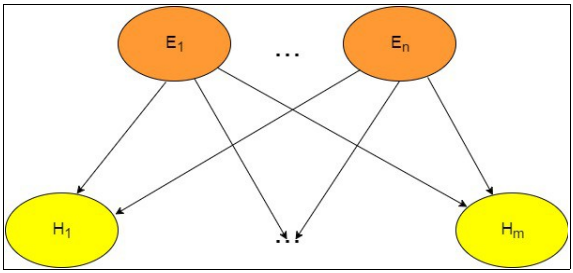
\includegraphics[scale=0.7]{imagenes/redes_bayesianas.png}
\caption{Grafo de una red bayesiana entre enfermedades y hallazgos}
\label{figura:red_bayesiana}
\end{figure}

Entonces el objetivo sería calcular las probabilidades del tipo:

$$
P({E}_{1}, {E}_{2}, \cdots, {E}_{n} | {H}_{1}, {H}_{2}, \cdots, {H}_{m})
$$

Estas probabilidades refieren a las probabilidades de cada enfermedad si están presentes o ausentes cuando se conoce una serie de observaciones asociadas a cada uno de los distintos hallazgos, entonces es necesario conocer:

\begin{itemize}
\item Probabilidad a priori de las distintas enfermedades
\item Probabilidad de que se obtengan determinadas observaciones asociadas a los distintos hallazgos conocida como la presencia o ausencia de las distintas enfermedades, es decir la verosimilitud.
\end{itemize}
En la cual integrando todas las probabilidades por la regla de Bayes se tiene:
$$
P({E}_{1},{E}_{2},\cdots,{E}_{n}|{H}_{1},{H}_{2},\cdots,{H}_{m}) = \frac{P({H}_{1},{H}_{2},\cdots,{H}_{m}|{E}_{1},{E}_{2},\cdots,{E}_{n})P({E}_{1},{E}_{2},\cdots,{E}_{n})}{\sum\limits_{{E}_{1}^{c},\cdots,{E}_{n}^{c} }^{}P({H}_{1},{H}_{2},\cdots,{H}_{m}|{E}_{1}^{c},{E}_{2}^{c},\cdots,{E}_{n}^{c})P({E}_{1}^{c},{E}_{2}^{c},\cdots,{E}_{n}^{c})}
$$
\subsection{Marco conceptual (palabras clave)}

\begin{itemize}
\item \textbf{Queratocono:} Transtorno corneal ectásico, caracterizado por adelgazamiento progresivo del estroma y debilitamiento estructural con protrusión apical en forma de cono, llevando a defectos refractivos como miopía progresiva, astigmatismo irregular, cicatrización y disminución de la visión \parencite{caruso2024corneal}

\item \textbf{Modelos bayesianos:} Modelos basados en la regla de Bayes en las cuales se estima la probabilidad a posteriori basada en información previa y verosimilitud de los datos \parencite{koski2011bayesian}

\item \textbf{Redes bayesianas:} Representación gráfica de dependencias para razonamiento probabilístico, en la cual los nodos son las variables aleatorias y representa dependencia directa entre las variables \parencite{sucar2006redes}
\end{itemize}


\subsection{Antecedentes empíricos de la investigación}
\subsubsection{Antecedentes Internacionales}
El estudio de \textcite{waddell2023applying} aplicó las redes bayesianas para el apoyo en la toma de decisiones, tomando datos de diferentes fuentes para explorar fenotípicos específicos y resultados clínicos, en la cual se pueden tener deficiencias debido al conjunto de datos pequeños y cohortes desequilibrados llegando a realizar inferencias falsas probabilísticas. Algo importante de destacar es como el uso de redes bayesianas ayuda en la detección de enfermedades especialmente en incertidumbre compleja, asimismo el autor indicar de que a pesar que la medicina actualmente se encuentra en competencia con el desarrollo de la inteligencia artificial, esta a su vez debe ser poder interpretada por los médicos en el cual el verdadero potencial de las redes bayesianas viene a ser la capacidad de hablar el lenguaje clínico, modelar preguntas relacionales causales y responder preguntas al explorar fenotipos individuales llegando a plantear preguntas cruciales como ¿por qué? y ¿que pasaria sí?. \\

El trabajo de \textcite{ferez2017redes} presenta una mejor evidencia de la medicina basada en la evidencia en el cual se debe tener un uso consciente, explícito y juicioso de la evidencia científica disponible para tomar la decisión de los pacientes, en el cual comprender la realidad y expresarla de manera sistemática, inteligible y sintética. Integrar la experiencia de los profesionales con la evidencia científica disponible para mejorar la toma de decisiones clínicas. Para conseguir este propósito se tienen diferentes entes matemáticas en la que su estudio enfatizó a las redes bayesianas como una de las herramientas más valiosas en el proceso de toma de decisiones. El trabajo planteo conceptos probabilísticos enfocado al análisis bayesiano en los cuales se fundamentan las redes bayesianas, para posteriormente crear dos redes a ejemplos prácticos, en la cual la red bayesiana tiene una capacidad para representar la relación causa entre variables involucradas en un problema y visualizarlas de una manera muy intuitiva, el cual es el modelo gráfico probabilístico más utilizado en el marco de la toma de decisión diagnóstica.

\subsubsection{Antecedentes Nacionales}
La investigación de \textcite{lopezmodelamiento} para optar el título de maestro en Estadística de la Pontífice Universidad Católica del Perú, se basó acerca de las infecciones respiratorias, en la cual buscó establecer una relación entre la incidencia de infecciones respiratorias agudas (IRA) y la incidencia de neumonía en el Perú en la cual además de ver si estas variables están correlacionadas quiso dar un enfoque espacial a nivel provincial en la cual se esperaría que la incidencia de (IRA) y neumonía sea mayor en provincias vecinas. Por lo cual se estudió la distribución espacial entre la incidencia de (IRA) y neumonía a nivel provincial en el Perú a través de un modelo espacial multivariado con efectos aleatorios condicionales autoregresivos utilizando inferencia bayesiana en el modelo jerárquico espacial multivariado a través del método de integración anidada de Laplace (INLA). El cual mostró una bondad de ajuste del modelo y su eficacia en la simulación realizada teniendo una optimización de tiempo menor, asimismo se vio una correlación positiva directa entre las personas con (IRA) sin neumonía y neumonía. Además de que se tuvo evidencia estadística entre las precipitaciones y la neumonía, indicando que el aumento de precipitaciones en una provincia reduce significativamente la incidencia de IRA sin neumonía, mientras el aumento de precipitación en una provincia aumenta la incidencia de neumonías en dicha provincia, teniendo una autocorrelación espacial moderada con respecto a las tasas de enfermedad entre provincias vecinas, recomendado que se puede trabajar con más covariables y factores que expliquen mejor la causalidad del modelo, de la misma forma incluir un modelo espacio-temporal empleando INLA que tiene una mejor eficiencia computacional al trabajar con más datos.

\section{Hipótesis y variables}
\subsection{Hipótesis general}
El enfoque bayesiano mejorará la detección y protocolo del queratocono

\subsection{Hipótesis específicas}
\begin{enumerate}
    \item Las variables más influyentes son las evaluadas en estudios previos de factores asociados al queratocono.
    \item El modelo jerárquico bayesiano que representa la relación entre variables viene a ser un multinomial ordinal beta.
    \item Las redes bayesianas representarán la relación causalidad del queratocono entre variables.
    \item El prototipo computacional apoyará en las inferencias de riesgo a nivel individual.
\end{enumerate}

\subsection{Identificación de variables e indicadores}
Las variables independientes viene a ser las probabilidades de generar queratocono en el nivel que se encuentre, asimismo como la clasificación de presencia o ausencia de esta enfermedad, que va a estar dependiendo principalmente de variables clínicas, demográficas y topográficas.

\begin{enumerate}
    \item \textbf{Variables dependientes}
    \begin{itemize}
        \item Probabilidad de generar queratocono.
        \item Clasificación de presencia o ausencia de queratocono. 
    \end{itemize}
    \item \textbf{Variables independientes} 
    \begin{itemize}
        \item Variables clínicas
        \item Variables demográficas
        \item Variables topográficas 
    \end{itemize}
\end{enumerate}

\begin{landscape} % Iniciar la página en formato horizontal
\subsection{Operacionalización de variables}

\begin{longtable}{p{4cm}p{6.5cm}p{5cm}p{3cm}p{2.5cm}}
    \caption{Matriz de operacionalización de variables} 
    \label{tab:matriz_operacionalizacion} \\

    \hline
    \textbf{Variable} & \textbf{Definición} & \textbf{Indicador} & \textbf{Tipo} & \textbf{Escala} \\
    \hline
    \endfirsthead

    \hline
    \textbf{Variable} & \textbf{Definición} & \textbf{Indicador} & \textbf{Tipo} & \textbf{Escala} \\
    \hline
    \multicolumn{5}{l}{\textbf{Independiente}} \\
    \hline
    \endhead

    \hline
    \endfoot

    \hline
    \endlastfoot

    \multicolumn{5}{l}{\textbf{Dependiente}} \\
    \hline
    Probabilidad de generar queratocono & Posibilidad de generar queratocono & Probabilidad queratocono & Continua & Razón \\
    \hline
    Presencia o ausencia de queratocono & Clasificación de la presencia o ausencia del queratocono & Presencia o ausencia & Dicotómica & Nominal \\
    \hline
    \multicolumn{5}{l}{\textbf{Independiente}} \\
    \hline
    \multirow{4}{*}{Variables clínicas} & \multirow{4}{6.5cm}{Variables tomadas en la revisión de la historia clínica usando test o cuestionarios.} & Ojo seco & Dicotómica & Nominal \\
    \cline{3-5}
    & & Alergias & Dicotómica & Nominal \\
    \cline{3-5}
    & & Frotamiento de ojos & Dicotómica & Nominal \\
    \cline{3-5}
    & & Antecedentes familiares con queratocono & Dicotómica & Nominal \\
    \hline \\
    \multirow{4}{*}{Variables demográficas} & \multirow{4}{6.5cm}{Información general de los pacientes} & Género & Dicotómica & Nominal \\
    \cline{3-5}
    & & Edad & Continua & Razón \\
    \cline{3-5}
    & & Altitud vive & Continua & Razón \\
    \cline{3-5}
    & & Clasificación altitud & Politómica & Ordinal \\
    \hline
    \hline \\
    \multirow{4}{*}{Variables topográficas} & \multirow{4}{6.5cm}{Son indicadores claves que se obtienen en los equipos de oftalmología de forma general} & Esfera topográfica & Continua & Intervalar \\
    \cline{3-5}
    & & Cilindro topográfico & Continua & Razón \\
    \cline{3-5}
    & & Eje topográfico & Continua & Razón \\
    \cline{3-5}
    & & Esfera manifiesta & Continua & Intervalar \\
    \cline{3-5}
    & & Cilindro manifiesto & Continua & Razón \\
    \cline{3-5}
    & & Eje manifiesto & Continua & Razón \\
    \cline{3-5}
    & & Emetropía & Politómica & Nominal \\
    \cline{3-5}
    & & Queratometria media & Continua & Razón \\
    \cline{3-5}
    & & Paquimetría & Continua & Razón \\
    \cline{3-5}
    & & Queratometria media & Continua & Razón \\
    \cline{3-5}
    & & BAD-D & Continua & Razón \\
    \cline{3-5}
    & & RMS & Continua & Razón \\
    \cline{3-5}
    & & IPP media & Continua & Razón \\
    \cline{3-5}
    & & Elevación frontal & Continua & Razón \\
    \cline{3-5}
    & & Elevación posterior & Continua & Razón \\
    \hline
\end{longtable}

\end{landscape}

\section{Metodología}
\subsection{Ámbito de estudio: localización política y geográfica}
El estudio se realizará en el centro de salud integral La Fuente en la ciudad del Cusco, ubicado en el distrito de San Jerónimo, provincia de Cusco, departamento de Cusco en el Perú.

\subsection{Tipo y nivel de investigación}
La investigación será de tipo aplicada no experimental retrospectivo ya que tomará en cuenta la información de los pacientes atendidos en el centro de salud en el año 2025 para evaluar los factores influyentes aplicando el análisis bayesiano de tal forma que se aumente el conocimiento científico acerca de la metodología estadística bayesiana y su aplicación. \parencite{hernandez2004introduccion}.
Asimismo el trabajo de investigación tiene un nivel relacional causal ya que se estudiará la relación y la causalidad que puedan tener las diferentes variables con respecto a la presencia del queratocono.

\subsection{Unidad de análisis}
La unidad de análisis serán los pacientes entre 10 a 40 años atendidos en el centro de salud integral La Fuente en el año 2025.

\subsection{Población de estudio}
La población de estudio serán todos los pacientes atendidos en el centro de salud integral la fuente que cumplan con los criterios de inclusión.

\subsubsection{Criterios de inclusión}
\begin{enumerate}
    \item Edad entre 10 a 40 años.
    \item Tengan información clínica de interés completa.
    \item Tengan información demográfica de interés completa.
    \item Tengan los exámenes topográficos de interés completos. 
\end{enumerate}


\subsection{Técnicas de recolección de información}
Las técnicas de recolección de información será a través de la revisión de documentos y/o análisis de datos secundarios, teniendo como instrumento la historia clínica y resultados del topógrafo de PENTACAM.

\subsection{Técnicas de análisis e interpretación de la información}
Los datos serán recopilados en un archivo de extensión \textsl{.xlsx} (Archivo Excel), en el cual los análisis se realizarán en el lenguaje de programación R bajo el entorno de desarrollo RStudio debido a su alta capacidad para manejar análisis estadístico desde los descriptivos hasta la realización de modelos robustos.

\subsection{Técnicas para demostrar la verdad o falsedad de las hipótesis planteadas}
Las hipótesis de investigación planteadas en el estudio serán comprobadas a través de los resultados a nivel inferencial que se obtenga mediante el modelo bayesiano establecido, asimismo por la inferencia que indiquen las redes bayesianas. Utilizando los criterios como es el criterio de AKAIKE (AIC), criterio bayesiano (BIC), entre otros.

\section{Presupuesto}


\begin{table}[htb]
\centering
\begin{tabular}{|p{7cm}|c|c|}
\hline
\textbf{RUBROS} & \textbf{COSTO(S/.)}& \textbf{TOTAL (S/.)} \\ \hline
\textbf{A) Recursos humanos:} & & \\
Laptop & 2000.00& \\
Papel bond A4 $80^0$ &100.00 & \\
USB &60.00&\\
Plumones cargador de plumones&50.00&\\
Corrector &10.00&\\
Lapiceros &30.00&\\
Documentos &100.00& 2 350\\ \hline
\textbf{B) SERVICIOS:} &&\\
Movilidad &500.00& \\
Tinta de impresora &240.00& \\
Impresión &150.00 &\\
Anillados &100.00&\\
Imprevistos &400.00& 1 390\\ \hline
& \textbf{TOTAL}& 3 740\\
 \hline
\end{tabular}
\caption{Presupuesto.}
\label{tabla:final2}
\end{table}


%%%%%%%%%%%%%%%%%%%%
%%%%%%%%%%%%%%%%%%%%%%%%%%%%%%%
%%%%%%%%%%%%%%%%%%%%

\section{Cronograma de la realización de la tesis}

\begin{center}
\begin{table}[htb]
\begin{tabular}{|p{4cm}|c|c|c|c|c|c|c|c|c|c|c|}
\hline
\multirow{2}{*}{\textbf{Actividades }} &\multicolumn{10}{c|}{\textbf{Fechas}} \\

 \cline{2-11}
 & \textbf{7-24} & \textbf{8-24} & \textbf{9-24}&\textbf{10-24}&\textbf{11-24}&\textbf{12-24}&
 \textbf{1-25}&\textbf{2-25}&\textbf{3-25}&\textbf{4-25}\\ \hline
 Revisión Bibliográfica & $X$ &&&&&&&&&\\ \hline
 Proyecto de Tesis &&$X$ &$X$&$X$&$X$&$X$&$X$&$X$&$X$&$X$ \\ \hline
 Capítulo 1 &&$X$ & $X$&$X$&$X$&$X$&&&&\\ \hline
Capítulo 2&&& &$X$&$X$& $X$& &&&\\ \hline
Capítulo 3 &&& &&$X$&$X$&$X$& & &\\ \hline
Conclusiones&&& &&&$X$&$X$&$X$&$X$& \\ \hline
Presentación y Revisión&&& &&&&&&&$X$\\ \hline
\end{tabular}
\caption{Actividades del proyecto de investigación}
\label{tabla:final}
\end{table}
\end{center}

\printbibliography[heading=bibintoc,title={Bibliografía}]

\begin{landscape}
\section{ANEXOS}
\subsection{Matriz de consistencia}
\begin{table}[h!]
\centering
\footnotesize
\begin{tabular}{|p{4.2cm}|p{4.5cm}|p{4.5cm}|p{3cm}|p{4.2cm}|}
\hline
\multicolumn{1}{|c|}{\textbf{Problemas}}  & \multicolumn{1}{c|}{\textbf{Objetivos}}  & \multicolumn{1}{c|}{\textbf{Hipótesis}} & \multicolumn{1}{c|}{\textbf{Variables}}   & \multicolumn{1}{c|}{\textbf{Metodología}} \\ \hline
\multicolumn{3}{|c|}{\textbf{General}}                               & \textbf{Dependientes}  & \multirow{4}{=}{
\begin{minipage}{4.2cm}
\justify
$\circ$ \textbf{Ámbito de estudio:} La Fuente Centro de Salud Integral - Cusco - Perú \\
$\circ$ \textbf{Tipo y nivel:} aplicada no experimental retrospectiva, relacional-causal\\
$\circ$ \textbf{Unidad de análisis:} Pacientes atendidos en el centro de salud integral\\
$\circ$ \textbf{Población:} Pacientes atendidos que cumplan los criterios de inclusión\\
$\circ$ \textbf{Muestreo:} Aleatorio simple\\
$\circ$ \textbf{Instrumento recolección de datos:}Historia clínica y resultados topográfico de PENTACAM\\
$\circ$ \textbf{Análisis e interpretación de datos:}Archivo de extensión \textsl{.xlsx} y RStudio.
\end{minipage}
} \\ \cline{1-4}
\multicolumn{1}{|p{4.2cm}|}{¿Cómo aplicar la metodología bayesiana en la detección del queratocono?} & \multicolumn{1}{p{4.5cm}|}{Desarrollar un protocolo de detección de queratocono bajo un enfoque metodológico bayesiano} & El enfoque bayesiano mejorará la detección y protocolo del queratocono & 
    \vspace{0.2cm}
    $\circ$ Probabilidad de presencia de queratocono\vspace{0.2cm}

    $\circ$ Clasificación de presencia o ausencia de queratocono\vspace{0.2cm}
  &                       \\ \cline{1-4}
\multicolumn{3}{|c|}{\textbf{Específicos}}                               & \textbf{Independientes} &  \\ \cline{1-4}
\multicolumn{1}{|p{4.2cm}|}{
    $\circ$ ¿Qué variables clínicas, demográficas y topográficas apoyan en la detección del queratocono?\vspace{0.2cm}

    $\circ$ ¿Qué modelo jerárquico bayesiano representa la relación entre las variables clínicas, demográficas y topográficas en la detección del queratocono?\vspace{0.2cm}

    $\circ$ ¿Cómo obtenemos la inferencia de probabilidad en la presencia o ausencia de queratocono a partir del modelo?\vspace{0.2cm}

    $\circ$ ¿Cómo implementar las inferencias de riesgo a nivel individual?} & \multicolumn{1}{p{4.5cm}|}{
    $\circ$ Determinar las variables clínicas, demográficas y topográficas que apoyen en la detección del queratocono.\vspace{0.2cm}

    $\circ$ Diseñar un modelo jerárquico bayesiano que represente la relación entre las variables clínicas, demográficas y topográficas en la detección del queratocono.\vspace{0.2cm}

    $\circ$ Construir una red bayesiana estructurada que infiera la probabilidad de presencia o ausencia del queratocono a partir de las variables observadas.\vspace{0.2cm}

    $\circ$ Implementar un prototipo computacional de inferencia de riesgo a nivel individual.

    } & \multicolumn{1}{p{4.5cm}|}{
    $\circ$ Las variables más influyentes son las evaluadas en estudios previos de factores asociados al queratocono.\vspace{0.2cm}

    $\circ$ El modelo jerárquico bayesiano que representa la relación entre variables viene a ser un multinomial ordinal beta.\vspace{0.2cm}

    $\circ$ Las redes bayesianas representarán la relación causalidad del queratocono entre variables.\vspace{0.2cm}

    $\circ$ El prototipo computacional apoyará en las inferencias de riesgo a nivel individual.\vspace{0.2cm}

    } & \multicolumn{1}{p{3cm}|}{
    \vspace{0.2cm}
    $\circ$ Variables demográficas.\vspace{0.2cm}

    $\circ$ Variables clínicas.\vspace{0.2cm}

    $\circ$ Variables topográficas.
    }  & \\ \hline
\end{tabular}
\end{table}

\end{landscape}

